% id: 25-22
% book: 100발100중 3-2 중간 · 01 3-2 중간(삼각비·삼각비의 활용·원과 직선·원주각·부록)
% section: 실전 문제 1회 · 서술형 문제
% figure: crop:fig-25-22.png
% answer: (1) $6\sqrt{3}\mkern3mu \mathrm{cm}$ (2) $3\sqrt{6}\mkern3mu \mathrm{cm}$
% answer_source: 답지(빠른정답)
% variant_level: 0 (원본 전사)
% 이 파일은 build.mjs 가 items.json 에서 만든다. 고칠 때는 items.json 을 고친다.
\smash{\raisebox{1.5mm}{\dmkichul{100발100중 3-2 중간 25쪽 22번}}}
\noindent\begin{minipage}[t]{0.58\linewidth}\vspace{0pt}\raggedright 그림에서 $\angle\pt{ABC}=\angle\pt{ADB}=90^\circ$, $\angle\pt{ABD}=45^\circ$, $\angle\pt{ACB}=60^\circ$이고, $\seg{AC}=12\mkern3mu \mathrm{cm}$일 때, 다음 물음에 답하고, 그 과정을 서술하시오. \mbox{[6점]}\end{minipage}\hfill\begin{minipage}[t]{0.4\linewidth}\vspace{0pt}\centering 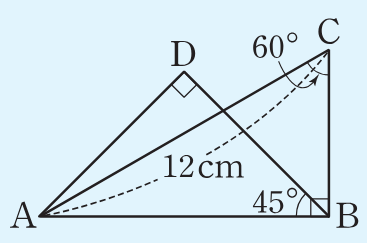
\includegraphics[width=88.0pt]{figures/fig-25-22.png}\end{minipage}\par
\dmsubprob{1} $\seg{AB}$의 길이를 구하시오. (3점)
\dmsubprob{2} $\seg{AD}$의 길이를 구하시오. (3점)
